%  Created by Branden Stone on 2015-01-15.
%  Copyright (c) 2015 Branden Stone. All rights reserved.
%--------------------------------------------------------
\documentclass{exam}


%---------------------------
% Packages
%---------------------------
\usepackage{amssymb, amsmath, latexsym, amsfonts, amsthm, mathrsfs} % Standard packages that are nice to have.
\usepackage{amsrefs} % Allows for easy referencing and citations.
\usepackage{verbatim} % Needed for \begin{comment} \end{comment}.
\usepackage[text={6in,9in},centering]{geometry} % Defines the dimensions of the text body.
\usepackage[colorlinks=true]{hyperref} % Allows for use of hyperlinks.
%\usepackage[doublespacing]{setspace} % Makes the document double spaced.
\usepackage[pdftex]{graphicx} % Allows for \includegraphics

\addpoints

\newcommand{\lst}[2]{#1_1,\dots,#1_{#2}}

%----------------------------
% Title and Author
%----------------------------

\title{Math 390 Midterm}
\author{Due Wednesday, April 6 at 5pm}
\date{}


%----------------------------
% Main Document Body
%----------------------------

\begin{document}


%-------------------------------------------------------------
% Front Matter: This is where you can add a table of contents,
% preface, list of figures, ETC. for this template we will 
% only create a title and author name with `\maketitle'
%-------------------------------------------------------------

\maketitle

\setlength{\parindent}{0em} % Sets indentation of new paragraph
\setlength{\parskip}{1em} % Sets space between paragraphs

%-------------------------------------------------------------
% Document Body: Essentially this is where you place the 
% content of your document. To use this template, just delete
% all of the text between here and the Bibliography Section.
% Then type whatever you desire.
%-------------------------------------------------------------

You must work completely on your own, consulting only the textbook, your course notes, and your homeworks as references. Show all of your work. If you have questions, you can come to my office hours or ask me via e-mail. Solutions should be written in \LaTeX\ or Markdown and converted to a PDF. There are \numquestions\ questions for a total of \numpoints\ points. Good luck!

\begin{questions}
	\question[36]  Let $G$ be a simple graph with edges $\lst e m$. The {\it line graph} $L(G)$ is the simple graph with vertices $\lst v m$ such that $v_i$ is adjacent to $v_j$ if and only if the edges $e_i$ and $e_j$ are adjacent in $G$.
	\begin{parts}
		\part Draw the line graph of $K_4$ and the line graph of $K_{2,3}$.

		\part Consider the following graph $G$.
		\begin{center}
			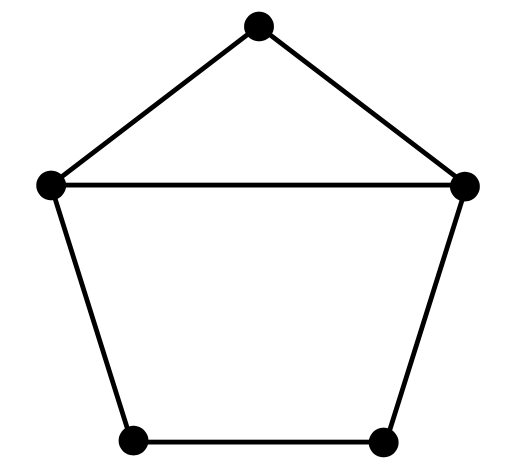
\includegraphics[width=0.15\textwidth]{mtpic1.png}
		\end{center}
		Does there exist a simple graph $H$ such that $L(H)=G$? If so, what is $H$?

		\part Determine the number of cycles of length 3 in the line graph of the Petersen graph.

		\part Let $G$ be a simple graph with degree sequence ($\lst d n$). Find a formula for the number of edges in $L(G)$ in terms of $\lst d n$. 
	\end{parts}

	\question[20] The following directed graph represents a city, with each edge of the graph corresponding to a street of the city. All of the streets are one-way streets in the indicated direction. After a snowstorm, a snow removal truck needs to start at the garage, drive down every street plowing snow, and end back at the garage.
	\begin{center}
			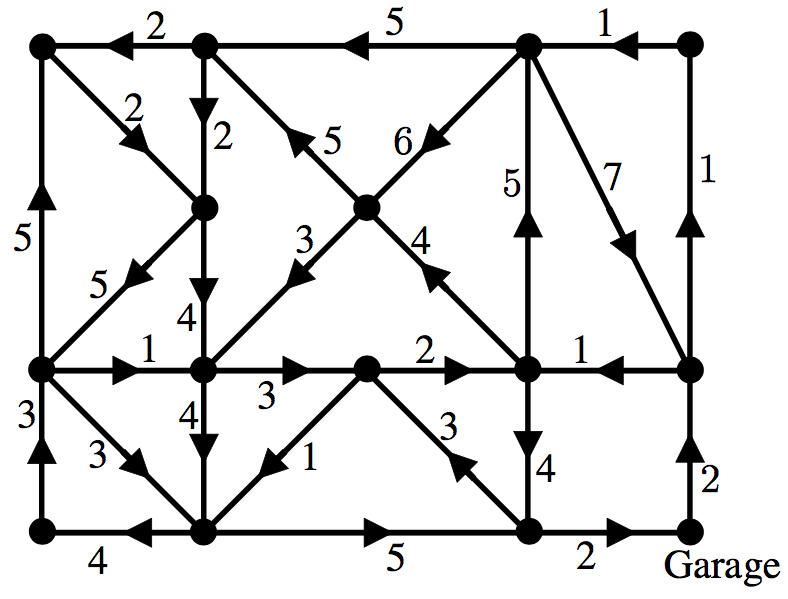
\includegraphics[width=0.5\textwidth]{mtpic2.png}
	\end{center}
	The edges are labeled with the length of time it takes to drive down the given street. Since the graph does not have an Eulerian trail, the truck will need to drive down some streets more than once. Determine the minimum amount of time required to plow all of the streets. Justify your answer.

	\question[24] Let $G$ be a simple planar graph with no cycles of length 3.
	\begin{parts}
		\part\label{parta} Use Euler's formula to prove that $G$ contains a vertex with degree 3 or less.
		\part Use part \eqref{parta} to prove that $G$ is 4-colorable without using the Four Color Theorem.
	\end{parts}

	\question[20] Let $G$ be a simple graph with $n$ vertices, and let $\overline G$ be the complement of $G$. (The complement of $G$ is defined on page 20 of Edition 4 and page 14 of Edition 5 of the textbook.) Use induction to prove that $\chi(G)+\chi(\overline G) \leqslant n+1$.


\end{questions}





\end{document}